% !TeX program = lualatex
\documentclass[]{article}

\usepackage{caption,subcaption,graphicx,float,url,amsmath,amssymb,amsthm,tocloft,cancel,thmtools,gensymb,braket,bm,tikz-feynman}
\usepackage[toc,nonumberlist]{glossaries}
\usepackage{glossaries-extra}
\usepackage[toc,page]{appendix}

\newcommand\numberthis{\addtocounter{equation}{1}\tag{\theequation}}

\newtheorem{thm}{Theorem}
\newtheorem{defn}[thm]{Definition}
\newtheorem{cor}[thm]{Corollary}
\newtheorem{lemma}[thm]{Lemma}
\graphicspath{{figs/}}
\widowpenalty10000
\clubpenalty10000
\setcounter{tocdepth}{2}
\tikzfeynmanset{compat=1.0.0}

%opening
\title{Theoretical Minimum\\Particle Physics 3\\Supersymmetry and Grand Unification}
\author{}

\begin{document}

\maketitle

\begin{abstract}
	These are my notes for the \emph{New Revolutions in Particle Physics 3--Supersymmetry and Grand Unification}\cite{susskind2010supersymmetry} lectures from Leonard Susskind's \emph{Theoretical Minimum} series\cite{susskind2007theoretical}. These notes follow on from \cite{susskind2010standard}. Feynman diagrams were prepared using \emph{TikZ-Feynman} \cite{ellis2016tikz}.
\end{abstract}

\tableofcontents
\listoffigures
\listoftables
\listoftheorems

\section{Renormalization  and dimensional analysis}

\subsection{Renormalization}

Most of the basic ideas of this quarter originated out of questions having to do with renormalization. Sometimes puzzles, sometimes useful observations about the renormalization of the standard model. I thought it would be a good idea to explain what renormalization is. It  is a combination of two things:
\begin{itemize}
	\item Learning how to eliminate out of the description of physics things arising from distances that are so small that they are irrelevant to the questions you are asking
	\item Learning how to think about how dimensional analysis tells you how to answer some of the difficult questions of quantum field theory field theory that have to do with distances much smaller than you might be interested in.
\end{itemize}

Examples of getting rid of things that are too small to be of interest.
\begin{itemize}
	\item Studying the nucleus aa protons and neutrons instead of quarks. Use QCD to figure out properties of protons and neutrons and their forces. Nucleons move slowly, so we can ignore relativity. Nucleus can be described by the non-relativistic theory of neutrons and protons. All we need from quark theory is to find out what the properties of protons and neutrons are--masses, spins, and the forces between them.
	\item For atoms, you might not be particularly interested in what makes up the nucleus. You use nuclear physics to calculate the properties of nuclei--which nuclei exist, their masses, and charges. Now we can forget protons and neutrons, but we need electrons.
	\item Now move on to atoms and forget their contents.
\end{itemize}

At each stage we eliminated the things what are smaller than we are really interested. The result is a coarse-grained description that is less accurate but more useful for our purposes.

The same thing is true in field theory. Each possible wavelength represents a degree of freedom. In describing things at one length scale we don't want to deal with shorter scales. We find a way to sum up the shorter stuff and replace by effective new parameters. That is all that renormalization is (plus some dimensional analysis).

\subsubsection{Example: atoms and atomic forces--going from atoms to molecules.}

Or going from nuclei + electrons to atoms, and how you deal with atomic forces: where do atomic forces come from? This isn't usually thought of as renormalization, but it is renormalization. Getting rid of the very small degrees of freedom, and also the very fast degrees of freedom: small usually goes with fast. The smaller a system is, typically the faster its motion is. So we are getting rid of small things and fast things.

Consider two atoms, each including a cloud of electrons. We want to get rid of the cloud of electrons, and all that very complicated stuff. We'd like to replace Figure \ref{fig:3-2-atoms} with two simple atoms with forces between them. The advantage is that the electrons are very fast compared to the nuclei. Nuclei are very heavy, starting at 2000 times the mass of the electron, so we could almost think of atom as a bowling ball with little flies surrounding it.

\begin{figure}[H]
	\begin{center}
		\caption{Two atoms with clouds of electrons}\label{fig:3-2-atoms}
		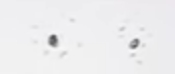
\includegraphics[width=0.5\textwidth]{3-2-atoms}
	\end{center}
\end{figure}

First approximation: the atoms are so heavy that they don't move at all. We want to calculate the effective potential between the two nuclei, in a way that gets rid of the electrons. Start by writing down Hamiltonian (ignore relativity, and some factors of $2\pi$).

\begin{align*}
	E=& \underbrace{\frac{P_1^2}{2M} + \frac{P_2^2}{2M} + \frac{e^2}{R_{12}}}_\text{protons} + \underbrace{\sum_i \frac{q_i^2}{2m} + \sum_{i,j}\frac{e^2}{r_{ij}}- \sum_i \frac{e^2}{R_{1i}} - \sum_i \frac{e^2}{R_{2i}}}_\text{things that involve electrons} \numberthis \label{eq:hamiltonian:H2}
\end{align*}

Intuitively there are two time scales here:
\begin{itemize}
	\item slow for nuclei, which are heavy;
	\item fast for electrons, which are a blur.
\end{itemize}

We'd like to get rid of the blur of electrons. This is easy to do \emph{in principle.} Take everything in the Hamiltonian that involves electrons; group them and think of them as the Hamiltonian for the electrons alone. Since the nuclei move slowly compared to electrons, treat them as fixed: to a first approximation nuclei are stationary.

To a first approximation fix the protons and treat the Hamiltonian as being for electrons in a fixed background from nuclei. We solve the Schr\"odinger equation for the lowest energy eigenvalue, $E_{electrons}(R_1,R_2)$. Then (\ref{eq:hamiltonian:H2}) becomes:


\begin{align*}
E=& \underbrace{\frac{P_1^2}{M} + \frac{P_2^2}{M} + \frac{e^2}{R_{12}}}_\text{protons} +\underbrace{ E_{electrons}(R_1,R_2)}_\text{Part of potential energy}\\
=& \frac{P_1^2}{M} + \frac{P_2^2}{M} + \frac{e^2}{R_{12}}+ E_{electrons}(R_1-R_2)
\end{align*}

We don't have to think about electrons again. All renormalization is based on this idea: getting rid of fast degrees of freedom, and replacing them with a renormalized Hamiltonian. 

What do we get rid of in Quantum Field Theory? Thins associated with very small distances, or things associated with high frequencies, or very short wave lengths (high energies). But first let's take a break and work on dimensional analysis.

\subsection{Dimensional Analysis}

In physics we have three scales, distance, time, and mass, and we can get rid of two of them by setting:
\begin{align*}
	c=&1\\
	\hslash=& 1
\end{align*} 
but we still need one dimension, which we will take to be a length (we could have used a time, or a mass). With the above units we have: 

\begin{align*}
	[m] =& [E]	= [P]\\
	[l] =& [t]	= \frac{1}{[m]}
\end{align*}

\subsubsection{A typical quantum field theory}

Renormalizing a scalar field $\Phi$. It has a Lagrangian, from which we derive Feynman diagrams. Our Lagrangian is:

\begin{align*}
	\mathcal{L} =& (\partial_\mu \Phi)^2 - V(\Phi) \text{, which we use to determine the \emph{action}}\\
	S =& \int d^4 x \mathcal{L} \text{, which has the same units as $\hslash=1$}
\end{align*}

This means that $\mathcal{L}$ has dimensions $[l^{-4}]$

\begin{align*}
	[(\frac{\partial \Phi}{\partial x})^2]=l^{-4} \text{, whence}\\
	[\Phi] = l^{-1}
\end{align*}

\subsubsection{Feynman digrams}

We imagine that the potential is something like:
\begin{align*}
	V(\Phi) =& \frac{m^2}{2} \Phi^2 + g \Phi^3 + \lambda \Phi^4 \numberthis \label{eq:potential}
\end{align*}
Since $[\Phi] = l^{-1}$ we can read off the dimensions of the coefficients:
\begin{itemize}
	\item $m$--mass;
	\item $g$--mass;
	\item $lambda$--dimensionless. Dimensionless copuling constants are very important in renormalization theory.
\end{itemize}

Feynman diagrams are built out of two types of elements:
\begin{itemize}
	\item vertices, read off from V--(\ref{eq:potential})-- see Figure \ref{fig:3-1-feynman-vertices}
	\item propagators: represent motion from one point to another--Figure \ref{fig:3-1-feynman-propagator}.
\end{itemize}

\begin{figure}[H]
	\begin{center}
		\caption{Elements of a Feynman diagram}
		\begin{subfigure}[t]{0.45\textwidth}
			\caption{Feynman Vertices for (\ref{eq:potential}). Cross in left hand vertex indicates absorption/re-emission. A Feynman diagram has a value, which corresponds to the amplitude for a process to happen.}\label{fig:3-1-feynman-vertices}
			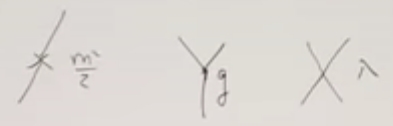
\includegraphics[width=\textwidth]{3-1-feynman-vertices}
		\end{subfigure}
		\begin{subfigure}[t]{0.45\textwidth}
			\caption{Propagator--amplitude that particle created at $x$ found at $y$. The line should not be read as a path along which particles moves, but rather as joining points where particle detected.}\label{fig:3-1-feynman-propagator}
			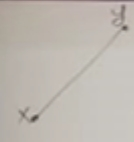
\includegraphics[width=\textwidth]{3-1-feynman-propagator}
		\end{subfigure}
	\end{center}
\end{figure}

\begin{itemize}
	\item We can represent the propagator is  $\braket{0|\Phi(y)\Phi(x)|0}$: create at $x$, annihilate at $y$.
	\item Dimension of propagator is $[l^-2]$. If there is no mass, distance between $x$ and $y$ is the only length scale in the problem--$\frac{1}{\lVert x-y \Vert^2}$. 
	\item If $x$ and $y$ close, propagator blows up--this is the source of all divergences in QFT.
\end{itemize}

Everything else is just building up Feynman diagrams, calculating them, and interpreting them.

Let's start with renormalization, and how it works in this very simple context.
Let's start with renormalization of the mass. Notice that (\ref{eq:potential}) contains $m^2$ -- usually mass only appears as $\sqrt{m^2}$. This is connected with $E=\sqrt{p^2 + m^2}$. So what is renormalization of $m^2$? What does it mean, and how do we do it? In Figure \ref{fig:3-1-feynman-vertices} we see that the interpretation of a mass term is just a basic simple Feynman diagram, a vertex in the digram where a particles is absorbed at a point and emitted from the same point. Does it have to be exactly the same point? If we have a microscope, an accelerator, which can resolve down to $10^{-17}m$, say, we aren't really interested in things that happen on smaller scales; so if we can find a process in nature that would mimic that vertex,  even if blurred, any process that absorbs and re-emits at a nearby point would be counted as part of mass term in an effective description in which we don't look too closely.

Are there any Feynman diagrams that we can build that will mimic a particle going in and a particle going out? We will build it out of the $\phi*4$ vertex in Figure \ref{fig:3-1-feynman-vertices}, the $\lambda$ vertex--see Figure \ref{fig:3-1-feynman-mimic}.


\begin{figure}[H]
	\caption{Mimicking the Vertex}\label{fig:mimicking:vertex}
	\begin{subfigure}[t]{0.3\textwidth}
		\caption{Particle emitted and returns to same point: scale so small we don't notice. Particle isn't going anywhere!}\label{fig:3-1-feynman-mimic}
		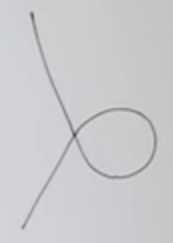
\includegraphics[width=\textwidth]{3-1-feynman-mimic}
	\end{subfigure}
	\begin{subfigure}[t]{0.3\textwidth}
		\caption{Amplitude following cut-off. We have reinstated $\lambda$ from $\phi^4$ term.}\label{fig:3-1-cutoff}
		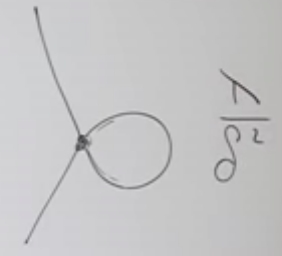
\includegraphics[width=\textwidth]{3-1-cutoff}
	\end{subfigure}
		\begin{subfigure}[t]{0.3\textwidth}
		\caption{Original mass term}\label{fig:3-1-original}
		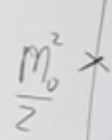
\includegraphics[width=\textwidth]{3-1-original}
	\end{subfigure}
\end{figure}

We saw in Figure \ref{fig:3-1-feynman-propagator} that the propagator has amplitude:
\begin{align*}
	\braket{0|\Phi(y)\Phi(x)|0}=&\frac{1}{|x-y|^2}\text{, which blows up to $infty$}
\end{align*}

Let us introduce a cut-off, saying that we are not interested in scales smaller than $\delta$; we smear the point over $\delta$--Figure \ref{fig:3-1-cutoff}. What is the amplitude in this approximation for a particle to come in, be absorbed, and re-emitted? There are two ways to make this happen. Figure \ref{fig:3-1-original} shows the original mass term. If we include Figure \ref{fig:3-1-cutoff} we see that the effect of ignoring terms smaller than $\delta$ is to increase the effective mass: the amplitude becomes $\frac{m_0^2}{2}+\frac{1}{\delta^2}$.  \emph{This is what we'd see in the laboratory if our resolution isn't high enough to resolve lengths less than $\delta$.}  

But we haven't finished. We haven't evaluated every possible Feynman diagram that can go into this. Let's do another Feynman diagram for the same thing. Figure \ref{fig:particles3-another-Feynman} depicts a particles going in and out, and something happening in the centre. What if the centre has size $\approxeq \Delta$? Can we integrate it out?

\begin{figure}[H]
	\begin{center}
		\caption{More diagrams from Figure \ref{fig:mimicking:vertex}}
		\begin{subfigure}[t]{0.45\textwidth}
			\caption{Another Diagram. Particle is absorbed where the heavy dot is. We need to integrate over all the places where it could be re-emitted. This derives from the third part of Figure \ref{fig:3-1-feynman-vertices}--4 things coming together at a vertex.}\label{fig:particles3-another-Feynman}
			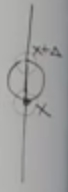
\includegraphics{particles3-another-Feynman}
		\end{subfigure}
		\begin{subfigure}[t]{0.45\textwidth}
			\caption{Diagram giving $\lambda^4$}\label{fig:particles3-yet-another-Feynman}
			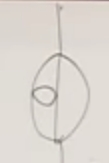
\includegraphics{particles3-yet-another-Feynman}
		\end{subfigure}
	\end{center}
\end{figure}

Coefficient is of order $\lambda^2$, so it is a second order Feynman diagram. It also has three propagators, each with coefficient $\frac{1}{\Delta^2}$, so $\frac{1}{\Delta^6}$. We need to integrate over all $\delta s$ 

\begin{align*}
	\lambda^2 \int_{\delta} \frac{1}{\Delta^6} d^4 \Delta \propto& \frac{\lambda^2}{\delta^2} \text{, by dimensional analysis.}
\end{align*}

There are many other Feynman diagrams, which will also contribute higher powers of $\lambda$

\url{https://youtu.be/W6srShxBCrk?t=2699}
	
\section{Fermions and bosons}

\subsection{Difference between Fermions and bosons}
Supersymmetry has to do with Fermions and Bosons, and their symmetries. We will Fermions and Bosons again, but, before that, we'll look at rotations.

Normally we are told that a rotation of $2\pi$ is equivalent to no rotation at all, but it is not true.

\begin{thm}[Rotation by $4\pi$ is equivalent to no rotation at all]
	Take a box, put a basketball in, and connect it to the walls with strings. A rotation by $2\pi$ tangles the strings; a rotation by $4\pi$ is equivalent to no rotation.
\end{thm}

Imagine that we have a particles, and we are interested in the spin $s$. What happens to the state when you rotate spin by $2\pi$.
\begin{itemize}
	\item apply string magnetic field and rotate;
	\item use field to precess particle.
\end{itemize}

Normally we'd expect it to come back to itself, but we know that $2\pi$ is not the identity. Perhaps it multiplies by a number. If we multiply by a phase, $\xi$, we won't be able to detect it. Multiplication by $4\pi$ squares phase, since it does nothing, so $\xi^2=1$, so $\xi=\pm1$.
\begin{align*}
	\ket{s} \rightarrow& +\ket{s} \text{, or}\\
	\ket{s} \rightarrow& -\ket{s}
\end{align*}

Can we detect this experimentally? It was long thought that we could not. If we take a family of electrons, all prepared identically, stick half into a magnetic field and rotate $2\pi$, we can't tell the two lots apart.

We can, however, do a 2 slit experiment\cite{aharonov1967observability}--Figure \ref{fig:particles3-2-2slit}.

\begin{figure}[H]
	\caption{A 2 slit experiment to detect rotation by $2\pi$}
	\begin{subfigure}[t]{0.45\textwidth}
		\begin{center}
			\caption{There is a magnetic field behind each slit, which traps electron temporarily. While an electron is trapped we rotate one field or the other, which can be detected in the interference pattern.}\label{fig:particles3-2-2slit}
			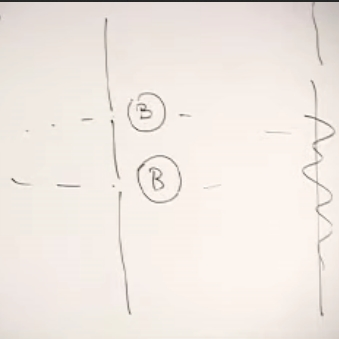
\includegraphics[width=\textwidth]{particles3-2-2slit}
		\end{center}
	\end{subfigure}
	\begin{subfigure}[t]{0.45\textwidth}
	\begin{center}
		\caption{We create a superposition of two states, electron going through slit 1 or slit 2. In either case electron is in one box or the other. Now we rotate 2nd box by $2\pi$. The wave function for an electron changes sign, but this has no physical consequence on it own. For the superposition, if we rotate one electron wave function, we can never find electron at centre. $\psi_1$ and $psi_2$ will interfere.}\label{fig:particles3-2-2slit-wave-function-2-2slit}
		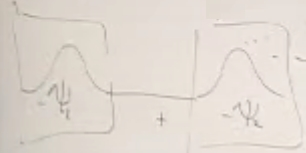
\includegraphics[width=\textwidth]{particles3-2-2slit-wave-function}
	\end{center}
\end{subfigure}
\end{figure}

The experiment has been performed for Fermions (which get the minus sign), and Bosons (which don't). The result is also deeply embedded in the theory.

You cannot interfere an up spin with a down spin: you can only interfere things that are otherwise the same.

\subsection{Feynman Diagrams}

We'll be dealing with diagrams in the vacuum, with nothing more complicated than a single closed loop--Figures \ref{fig:particles3-2-loops} and \ref{fig:particles3-2-loops-boson}. This diagram controls, among other things, the amplitude that you start with nothing and get nothing. It is part of the vacuum structure. The diagram has a  value, which is a contribution to the vacuum energy. Just as Figure \ref{fig:particles3-2-loops-p} contributes to the energy of the particle, Figure \ref{fig:particles3-2-loops} and \ref{fig:particles3-2-loops-boson} contributes to the energy of the vacuum. Does it shift it up or down? Surprisingly the answer is different for Fermions and Bosons.


\begin{figure}[H]
	\caption{Closed Loops Feynman diagrams}
	\begin{subfigure}[t]{0.3\textwidth}
		\caption{Fermion Closed Loop}\label{fig:particles3-2-loops}
		\feynmandiagram{
			b-- [fermion,half left]
			c-- [fermion,half left] b
		};
	\end{subfigure}
	\begin{subfigure}[t]{0.3\textwidth}
		\caption{Boson Closed Loop}\label{fig:particles3-2-loops-boson}
		\feynmandiagram{
			b-- [boson,half left]
			c-- [boson,half left] b
		};
	\end{subfigure}
	\begin{subfigure}[t]{0.3\textwidth}
		\caption{Loop for particle}\label{fig:particles3-2-loops-p}
		\feynmandiagram[vertical=e4 to e1]{
			e1[particle=$e^-$]--[fermion]e2--[fermion]e3
			--[fermion]e4[particle=$e^-$],
			e2--[photon,looseness=3.0,half left]e3
		};
	\end{subfigure}
\end{figure}

\begin{thm}[Contribution of loops to vacuum energy]
	The contribution to the vacuum energy of a loop of Bosons is positive;
	The contribution to the vacuum energy of a loop of Fermions is negative.
\end{thm}

\begin{proof}
	You can think of a loop as the production and annihilation of a pair, or as a single particle looping in space-time. The sign of a particle in a loop can be either positive or negative. What about two loops--Figures \ref{fig:two:loops:fermion} and \ref{fig:two:loops:boson}? This is the product of two separate loops. So if there is a plus sign for one loop, there will be a plus sign for the product: if there is a minus sign for one loop, there will still be a plus sign for the product. So there will  be a plus sign for the product either way.
	
	\begin{figure}[H]
		\caption{Two loops}\label{fig:two:loops}
		\begin{subfigure}[t]{0.5\textwidth}
			\caption{Two Fermion loops}\label{fig:two:loops:fermion}
			\feynmandiagram{
				b-- [fermion,half left]
				c-- [fermion,half left] b
			};
			\feynmandiagram{
				b-- [fermion,half left]
				c-- [fermion,half left] b
			};
		\end{subfigure}
		\begin{subfigure}[t]{0.5\textwidth}
			\caption{Two Boson loops}\label{fig:two:loops:boson}
			\feynmandiagram{
				b-- [boson,half left]
				c-- [boson,half left] b
			};
			\feynmandiagram{
				b-- [boson,half left]
				c-- [boson,half left] b
			};
		\end{subfigure}
		\begin{subfigure}[t]{0.45\textwidth}
			\caption{Two Fermion loops, split at t=0}\label{fig:two:loops:split}
			\begin{equation*}t=0
				\feynmandiagram[inline=(c.base),horizontal'=a to c]{
					a -- [quarter left]
					b-- [quarter left]
					c-- [quarter left]
					d-- [quarter left] a,
				};\,
				\feynmandiagram[inline=(c.base),horizontal'=a to c]{
					a --[quarter left]
					b-- [quarter left]
					c-- [quarter left]
					d-- [quarter left] a,
				};
			\end{equation*}		
		\end{subfigure}
		\begin{subfigure}[t]{0.45\textwidth}
			\caption{Two Fermion loops, interchange}\label{fig:two:loops:interchange}
			\begin{equation*}t=0
				\feynmandiagram[inline=(c.base),horizontal'=a to c]{
					a -- [quarter left]
					b-- [fermion,quarter left]
					c-- [quarter left]
					d-- [quarter left] a,
				};
				\feynmandiagram[inline=(c.base),horizontal'=a to c]{
					a --[quarter left]
					b-- [quarter left]
					c-- [quarter left]
					d-- [anti fermion,quarter left] a,
				};
			\end{equation*}		
	\end{subfigure}
	\end{figure}
	Let's assume our particles are Fermions: lets break the loop and look in the middle at t=0--Figure \ref{fig:two:loops:split}. 
	\begin{itemize}
		\item What happens for amplitude of a system if we exchange two Bosons? Plus sign. 
		\item What happens for amplitude of a system if we exchange two Fermions? Minus sign. 
	\end{itemize}
	Now interchange particles, as in Figure \ref{fig:two:loops:interchange}.
	\begin{itemize}
		\item If we are dealing with Fermions we get a minus sign. We have gone from two loops (positive) to one loop, negative.
		\item If we are dealing with Bosons we get a plus sign.
	\end{itemize} 
\end{proof}

The consequences are profound:
\begin{itemize}
	\item the contribution to the vacuum of a Boson loop is positive;
	\item the contribution to the vacuum of a Fermion loop is negative.
\end{itemize}
We have this strange puzzle about the vacuum energy; it is extremely small, and we call it Dark Energy. The naive calculation in quantum field theory would give an answer 123 orders of magnitude larger.  We saw that the answer can be positive or negative: it depends on all sorts of things, such as mass and charge. We can at least get positive and negative signs. The fact that they cancel to 123 order of magnitude is bizarre, but we can cancel. All things being equal, a boson and a fermion will give exactly the same contribution, except for a different sign.

That doesn't mean that the vacuum energy is zero, but it suggest that maybe there is a lot of cancellation. To get an exact cancellation, we'd need for every boson with the same mass and same properties, then we could conceive that the particles would cancel out the vacuum energy.

We know that there isn't an exact Boson for each Fermion. For example, the electron: there isn't a Boson equivalent to the electron: if there were, the partners could be produced--Figure \ref{fig:partners}-- with exactly the same probability as an electron-positron pair--Figure \ref{fig:re:emit}. We know this isn't the case: Nature does not have a Boson$\leftrightarrow$Fermion symmetry.

\begin{figure}[H]
	\begin{center}
		\caption{Why there isn't a Boson equivalent to the electron}
		\begin{subfigure}{0.45\textwidth}
			\caption{Producing the partners}\label{fig:partners}
			\feynmandiagram[vertical'=b to a]{
				i1 [particle=\(e^{-}\)]
				-- [fermion] a
				-- [fermion] f1 [particle=\(e^{-}\)],
				a -- [photon,edge label=\(\gamma\)] b,
				i2 [particle=\(e^{+}\)]
				-- [boson] b
				-- [boson] f2 [particle=\(e^{+}\)],
			};
		\end{subfigure}
		\begin{subfigure}{0.45\textwidth}
			\caption{Reemitting the Fermions}\label{fig:re:emit}
			\feynmandiagram[vertical'=b to a]{
				i1 [particle=\(e^{-}\)]
				-- [fermion] a
				-- [fermion] f1 [particle=\(e^{-}\)],
				a -- [photon,edge label=\(\gamma\)] b,
				i2 [particle=\(e^{+}\)]
				-- [fermion] b
				-- [anti fermion] f2 [particle=\(e^{+}\)],
			};
		\end{subfigure}
	\end{center}
\end{figure}

 Keep these two thoughts in mind.
\begin{itemize}
	\item  However, if we had a theory which was sufficiently symmetrical, we would at least have a chance of cancelling the vacuum energy.
	\item Can this also help with the self-energy of Bosons: we have quadratic infinities. Even if the initial mass is zero, we have diagrams that give us a huge mass.
\end{itemize}

Fermions don't have same problem with infinities. Now consider Figure \ref{fig:2loops}. In Figure \ref{fig:2loops:bosons} we have a Boson going round the loop, and in Figure \ref{fig:2loops:fermions} a Fermion. Fermion and Bosons always have opposites signs, so we can imagine, if everything were absolutely symmetrical, we might imagine things cancelling, so that self energy is not infinite.

\begin{figure}[H]
	\caption{Two loops for a boson}\label{fig:2loops}
	\begin{subfigure}{0.45\textwidth}
		\caption{Boson going around loop}\label{fig:2loops:bosons}
		\feynmandiagram[vertical=b to d]{
			i--[boson]b,
			a --[boson,quarter left]
			b-- [boson,quarter left]
			c-- [boson,quarter left]
			d-- [boson,quarter left] a,
			ii--[photon]d	
		};
	\end{subfigure}
	\begin{subfigure}{0.45\textwidth}
		\caption{Fermion going round loop}\label{fig:2loops:fermions}
		\feynmandiagram[vertical=b to d]{
			i--[boson]b,
			a --[quarter left]
			b-- [quarter left]
			c-- [quarter left]
			d-- [quarter left] a,
			ii--[photon]d	
		};
	\end{subfigure}
\end{figure}
\url{https://youtu.be/-nBOCF0sPgU?t=2110}

\section{Propagators and renormalization of mass}

TBP

\section{Symmetry and Grassmann numbers}

TBP

\section{A first supersymmetric model}

TBP

\section{Supersymmetry building blocks}

TBP

\section{Lagrangians that preserve supersymmetry}

TBP

\section{Generalizing supersymmetry to 3+1 spacetime, and QFT}

TBP

\section{Supersymmetry breaking and an introduction to grand unified theories}

TBP

\section{GUTs, the SU(5) representation, proton decay}

TBP


\bibliographystyle{unsrt}
\addcontentsline{toc}{section}{Bibliography}
\raggedright
\bibliography{tm}

\end{document}
